% ==== Introduction ====
\section{Introduction}

\begin{frame}{Definitions: ill-formed}
  \begin{block}{Ill-formed [defns.ill.formed] [defns.well.formed]}
    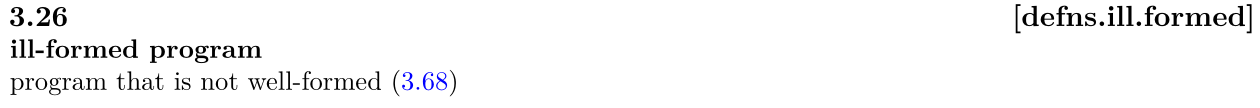
\includegraphics[width=\textwidth]{img/cplusplus_draft/defns.ill.formed.png}\\[1em]
    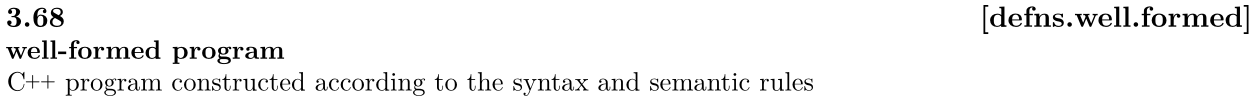
\includegraphics[width=\textwidth]{img/cplusplus_draft/defns.well.formed.png}

    \vspace{1em}
    {\bfseries Ill-formed, no diagnostic required:} program is ill-formed, but no compiler diagnostic is required, e.g. different definitions for an inlined function.
  \end{block}
\end{frame}

\begin{frame}{Definitions: Undefined Behavior (UB)}
  \begin{block}{Undefined behavior (UB) [defns.undefined]}
    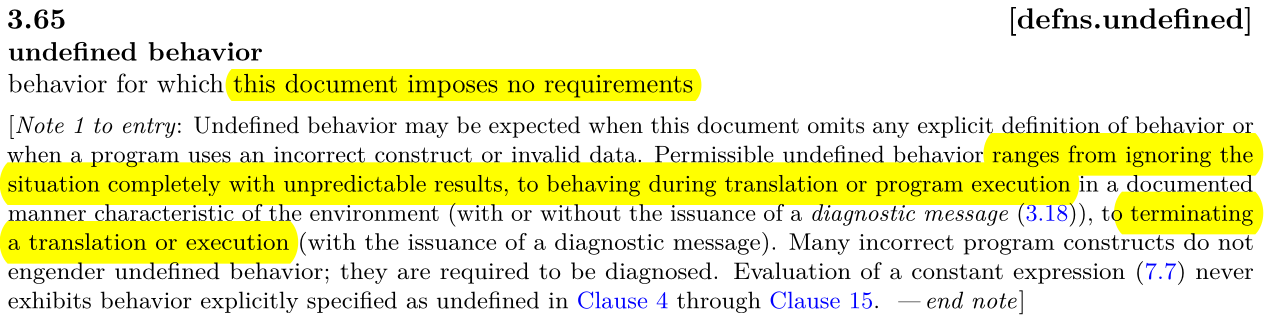
\includegraphics[width=\textwidth]{img/cplusplus_draft/defns.undefined.png}
  \end{block}
\end{frame}

\begin{frame}{Definitions: Type punning}
  \begin{itemize}
  \item From Wikipedia\footnote{Source: \url{https://en.wikipedia.org/wiki/Type_punning}.}: \textit{``In computer science, a type punning is any programming technique that subverts of circumvents the type system of a programming language in order to achieve an effect that would be difficult or impossible to achieve within the bounds of the formal language.''}
    \begin{itemize}
    \item I.e., accessing \textbf{underlying in-memory representation} of an object of type \inlineCode{Foo} as a different type, \inlineCode{Bar}, e.g.\\[1ex]
      \tikz[uint32_t/.style={draw,rectangle split,rectangle split parts=4,rectangle split horizontal,minimum width=4in,minimum height=20pt,inner xsep=7pt}]{

  \node[uint32_t,label={below:\texttt{uint32\_t}}] (uint32t) {};
  \node[right=10pt of uint32t] {\ldots and accessing as \texttt{unsigned char[]}}

}

    \end{itemize}
    \bigskip
    \bigskip

  \item \alert{Why?} Useful for (de-)serialization, networking code, or calling legacy (C) library code.
  \end{itemize}
\end{frame}

\begin{frame}{\texttt{reinterpret\_cast} and UB}
  As we saw, some \texttt{reinterpret\_cast}s result in UB\ldots\\[2em]

  Q: Why, C++, why?~\worried\\
  \pause
  A: TL;DR\footnote{There are more causes; but this is a nice summary.}: Can two pointers of \textbf{different types} really point to the \textbf{same object}?\\
  Compiler may optimize based on that!
\end{frame}
